
%Chapter Overview

\section{Introduction}
The aim of the literature review section of this or any dissertation is to show that the author has indeed researched, understood, and has a good grasp of, the main work concerning the chosen topic or question in your field. This work can be done by searching online for websites, papers, and books that can be used to further enhance the knowledge of the topic at hand. The review is guided by one’s research objective or by the issue or thesis someone is trying to argue out that will also provide the framework for one’s further work. 
\newline
\newline
This article focuses on precisely that. It provides a look into Point of Sale and inventory management systems and their relation and impact in the restaurant industry as well as other industries where they can be adopted too.
\newline
\newline
Today we are seeing a huge shift in restaurant technology. From touch screen ordering systems at tables to kiosks that you can order food and go to collect it, restaurateurs across the world are using new, modern devices to keep their restaurants on the cutting edge of the industry. According to Grand View Research, the global point-of-sale (POS) terminals market size in 2019 was USD  69.0 billion and is expected to reach USD 125.9 billion by 2027[fig].

\begin{figure}[h!]
	\caption{Bar chart showing the increase in value of the POS terminal market size.}
	\label{image:myImageName}
	\centering
	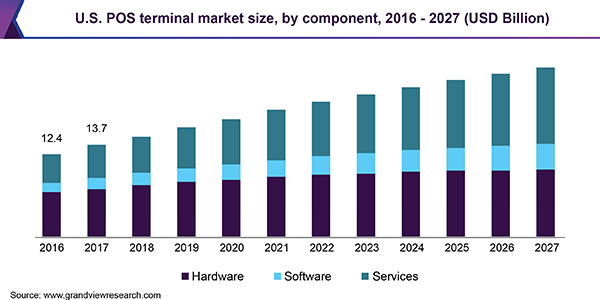
\includegraphics[width=0.9\textwidth]{Fig images/us-pos-terminal-market.png}
\end{figure}

This proves that the market shows no sign of slowing down. Where you can buy goods there is always a need for a stock management/POS system. 
\newline
\newline
With new technology, the interaction between customers and members of staff is dramatically reduced thus creating a new challenge for business owners. Customer service is still a vital part of a business and keeping customers coming back. Superior customer service is at the heart of every great restaurant, and new restaurant technologies can give restaurants an edge in responding to customer needs (Strong 2013). If a customer’s only interaction with staff is to pay, then this part of the process has to be as efficient as the rest of the experience, and having a fast and reliable POS system allows this. 
%%%%%%% whats strong 2013

\section{What is a Management System?}
Management systems are systems that allow restaurant owners /managers to manage their stock levels through a piece of software linked from a computer to the point of sale system. They assist owners in tasks such as avoiding overstocking, avoiding running out of stock, overall sales, customer sales and staff sales. A well designed and reliable system is essential to any business. It therefore helps the user make key decisions on whether to keep products or not, whether to reach out to a customer that hasn't been to your restaurant in a while and to review staff sales to see if they are doing their work correctly. Being able to make these well-informed decisions leads to increased profits along with greater stock management.

\section{History of inventory management}

Up until recently manual ordering in restaurants was used. Notepad and pens and basic point of sale systems were very common. Each order was taken then rang up on the till and the order sheet was then handed into the kitchen. This was a very time consuming and inefficient task which cost owners money and prolonged the time it took for customers to get their order. This was not too dissimilar to retail outlets from the past.
\newline
\newline
Many years ago, in retail outlets, workers wrote down every sale to keep a record and calculate it all up then check against stock levels at the end of every day. This was a time consuming and a very tedious task which was added to the end of every workday. This work was highly skilled as it had to be exact or there would be an imbalance. This imbalance could be found in small retail operations so the room for human error in a big business could be massive. 
\newline
\newline
After the Industrial Revolution, efficiency and mass production became the main goals of businesses, along with improved customer experience at the point of sale (Miller,1997). In the early 1930s, the first modern check-out system was designed. Punch cards that corresponded with catalog items were used to process transactions. The cards were read through a computer which then passed the product information to the storeroom. Items were then brought from the back up to the customer finally the transaction was complete. This system revolutionized stock control. Now business owners were able to keep track of all sales as well as generate billing records and manage their inventory. This greatly reduced the risk of stolen stock as well as saving on man-hours.
\newline
\newline
While it saved owners money and time, the punch card system was an expensive one. Merchants needed a better system therefore researchers created one. In the late 1940s and early 1950s, researchers created the first bar-code system. It used ultraviolet light-sensitive ink and a reader to mark items for sale.

\begin{figure}[h!]
	\caption{Patent of the original bar-code scanner.}
	\label{image:myImageName}
	\centering
	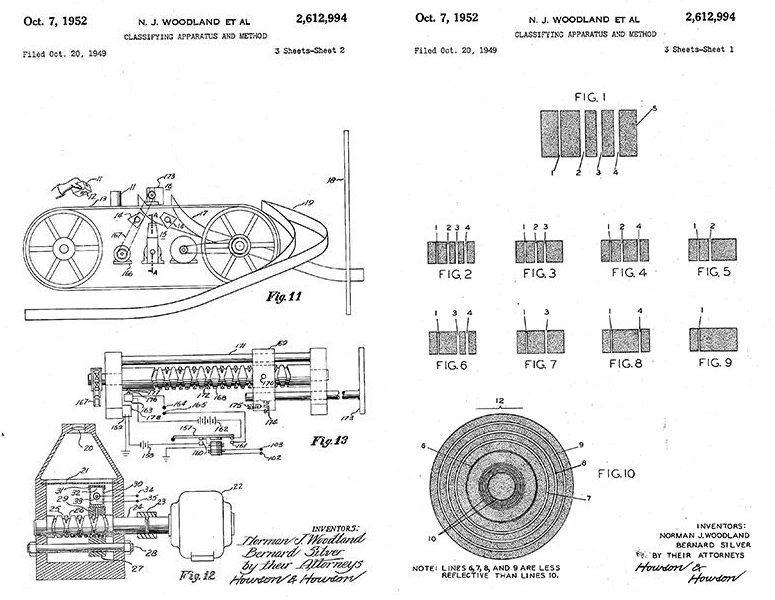
\includegraphics[width=0.9\textwidth]{Fig images/patent.png}
\end{figure}

Once again, the system was too expensive and lacked the computing power needed to make it work. While retailers knew what they needed to keep tabs on their stock levels, society simply lacked the resources and computing power to make any great strides into the field, and thus the concept stalled, and progress was nonexistent.
\newline
\newline
In the 1960s the development of affordable laser technology revived the concept of an efficient stock management system. Lasers technology allowed for the manufacturing of smaller, faster, and cheaper scanners. In the late 1960s the bar code, or the Universal Product Code (UPC) as it was called at the time, was developed. With vast improvements in computing power, the ability of UPC codes to help track and manage inventory improved exponentially.
\newline
\newline
During the 1990s, due to advances in computer and software technology, retailers began implementing modern inventory management systems. Modern inventory management systems must have the ability to track sales and available stock levels. They also must be able to provide up to date information for the owner to make key decisions regarding purchasing.

\section{Role of inventory management}

Inventory often represents a significant portion of a business’s operational revenue. According to the Oxford dictionary, inventory control is defined as the fact or process of ensuring that appropriate amounts of stock are maintained by a business, to be able to meet customer demand without delay while keeping the costs associated with holding stock to a minimum.

\begin{figure}[h!]
	\caption{Inventory Control}
	\label{image:myImageName}
	\centering
	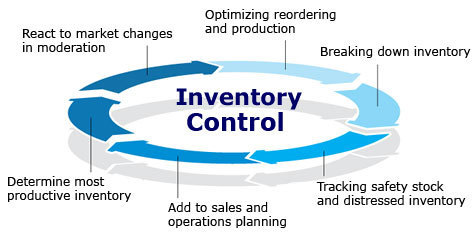
\includegraphics[width=0.9\textwidth]{Fig images/inventory-control.jpg}
\end{figure}

Stock levels must be kept adequately controlled to allow a business to offer customers the best possible service. If a customer visits any retail outlet to purchase a product but that product is sold out it could lead to them never returning. Owners and management need to ensure that adequate forecasting is maintained to complete all sales, especially in such a competitive market as we see today. This is especially important in the restaurant trade. An owner will always want enough items in stock to fulfill any orders it receives although they do not want to have excessive stock levels which will result in food being thrown out. This costs money which could inevitably destroy the business. The goal of any well-run business is to have all choices available to customers but not have excessive amounts of leftovers. Although the concept appears simple, it requires careful planning, standardized procedures, and monitoring to achieve desired results \cite{INV}.

\section{Impacts of inventory management systems include:}

\subsection{Customer satisfaction}

If a management system is used to the best of its capabilities, then stock levels are always kept to a happy medium in which any product is there to be purchased at any time. Owners can analyze product sales in real-time and make key, well-informed decisions that let the running of business seem almost effortless. Owners can have their popular items in stock ready to instantly fulfill any order. They can also analyze past sales to adequately forecast what sells and on what occasion. This will result in gaining a good reputation among the general public as being reliable hence bringing in repeat custom.

\subsection{Pricing}

Having good stock management reduces the chance of stock waste. This will result in the saving of a lot of money. Keeping stock at a good operating level will keep business costs down and in turn, keep the costs of the customer down. 

\subsection{Maximizing efficiency}

Maximizing efficiency is a key objective for this project. This was not only an important aspect of the POS part of the project but of the business management side of it too. A good management system will not only affect the price of items but will help in the handling and storage aspects of business too along with having the right staff on when deliveries are coming in. Knowing everything you need to know will result in products finding its way to the customer as quickly and as efficiently as possible. The inventory doesn’t need to be counted.

\subsection{Financial management}

Improved financial control is one of the most important goals of inventory management systems. A well-designed Management System will ensure the maximum value is generated from purchased stock. In addition to the actual cost of acquiring inventory, costs are associated with transporting and storing inventory[fig].
%\begin{figure}[h!]
%	\caption{Financial Management.}
%	\label{image:myImageName}
%	\centering
%	
\includegraphics[width=0.9\textwidth]{Fig images/notsure.jpg}
%\end{figure}

These costs are called carrying costs.

\subsection{Menu planning}

Menu planning is a key part of any restaurant. An owner needs to know what’s selling and what isn’t. There is no point in having stock that isn’t selling left there and going out of date only to have to order more of the same stock in. Decisions need to be made on every under-performing item on the menu. This requires considerable planning to ensure that menus are as cost-effective as possible while also providing customers with what they want at prices they will purchase them at.

\subsection{Forecasting and ordering}
Forecasting can greatly affect inventory control. Bad forecasting can lead to excess ordering thus tying up a lot of money in inventory. This will, in turn reduce the cash flow of the business and lead to a lot of waste of stock. 
                    
\section{Advantages of a Management System}

Management systems offer up to date sales figures along which can be used to gauge the performance of all products on sale. While the need for hand counting stock will always be there to ensure your business isn’t being robbed or people aren’t making mistakes, management systems still make the life of the owner a lot easier.

\subsection{Speed and Efficiency}

An up to date sales form can be formed in seconds, giving the owner all the information, they need on anything. This saves on time, money, and man-hours that can be directed at other areas of the company.

\subsection{Document Generation}

Receipts can be generated at the click of a button allowing the user to document all sales, Secondly the user can generate excel sheets of data ranging from reports and graphs that are created as sales and transactions are made.

\section{Disadvantages of a Management System} 

\subsection{Reliance on Technology}

Using a computerized management system, while extremely useful, poses some disadvantages. One is an over-reliance on technology, Outside factors like power failures or the loss of Internet connection or network connectivity can render the system useless. This can lead to loss of earnings and customer dissatisfaction.

\subsection{Accuracy Issues}

A computerized management system alone does not ensure accuracy. A system and its data are only as good as the information passed into it. If a member of staff makes a mistake this could have serious ramifications down the line. Inaccurate stock and cash levels could be detrimental to a company as well as compromising the integrity of the reports it generates. This is why a plan must be put in place to be able to validate their data and check the figures reported by the system.

\subsection{Risk of Fraud}

Any computerized system carries the risk of fraud. An inventory management system is no different. The system could be hacked at the gain of someone looking to benefit from a company that relies on its management system to conduct its day to day business.

\section{Areas of further research}

Artificial intelligence could play a huge part in the future of Management and POS systems. The technology consolidates, standardizes and enriches data, providing the foundation for AI analytics to present data-driven recommendations that managers can either chose to accept, reject or revise\cite{AI}
\newline
 While it has already been implemented in a very small number of systems, automatic stock ordering and forecasting using AI could be beneficial in helping owners run the business. Menu decisions could be made by the system which would take all the data it has access too and make well-informed decisions based on such data.
\newline
\newline
While this could be deemed an area of further research it could also be deemed an area of controversy. AI could take the decision making out of the hands of the owner and put it into the hands of the technology. Eliminating the human decision-making process could affect companies. While there are great strides in computing power you would always need a person to make the final call. Eliminating human interaction would be impossible as sales, stock, and money levels will always have to be cross-checked against any information a management system has. This leads to the question, is AI in inventory management an inevitability or a luxury we don’t need?

\section{Users}

Business Management Systems are everywhere. You can easily spot these systems in areas such as shops, bars, clubs, and restaurants. They are needed by every business with a considerable amount of daily sales. While our Management System is intentionally built for restaurants it can be easily incorporated into any business. The software can easily be adopted anywhere there are needs similar to our system with no tweaking at all. This has been achieved by carefully reviewing different models and usability of the proposal in different case studies.
\newline
\newline
As a result, the system was designed to be flexible in its application thus allowing anyone to use it in any business premises. With all this said and done, the users of this particular system would-be owners, management, waiting for staff, chefs, and bar staff.

\section{Use Cases}

The following use case illustrates the usability of the software based on the users identified above. While the use of the system may vary, we have listed the predominant features of the system which are universally essential. This further illustrates the importance of incorporating the functionality of POS systems and RMS into one. Not only does it provide grounds for reusable codes it as well provides grounds for upgrades involving:
\begin{itemize}
    \item blockchain and the Internet of Things.
    \item Owner Management and Till Application
    \item Management Management and Till Application
    \item Waiting Staff Restaurant Application
    \item Chefs Kitchen Ticketing Application
    \item Bar Staff Till Application
\end{itemize}

\section{Project Platform}
A restaurant management system must have the ability to work on any machine regardless of settings and Operating System. We therefore built this system as a standalone system which could be installed any machine. This improves on re-usability of the code while easing the task of upgrading in the future. 
As illustrated above, we used PHP as the main language for the project. PHP is platform independent and runs on any Operating System. When deciding on the language, we reviewed the ease in which it is maintained, its performance and scalability. These were the deciding factors in the project review. PHP therefore was selected as the best language to learn and incorporate into the project based on our timeline and project requirements.

\section{Project Software}

The following is a list of the software we used for our project and why we decided to use it. For the most part we put together a list of what we needed at the start of the project and decided on what piece of software we would use for each specific job. 

\subsection{Xampp}

XAMPP is a free and open-source cross-platform web server solution that we used to develop this project \cite{XAMP}. Throughout our four years in college we predominantly used WAMP for our web servers. While WAMP would be efficient enough to build on our Windows laptops we wanted to use a server that was cross platform so our program could be run on any Operating System. XAMPP offered us exactly this so it was the obvious choice.

\subsection{Visual Studio Code}

For our code editor we used Visual Studio Code. VS Code is a light weight software with an embedded Git control which is the main reason we chose to work with it \cite{VSC}. We also looked at the idea of using sublime text but VS Codes reliability along with its ease of file creation made it our first choice. VS Code has everything we needed to build this project including Git integration and in-built terminal for an all in one experience.

\subsection{MySQL}

MySQL is an open-source relational database management system \cite{SQL}. Its reliability and high performance were among the reason we chose it, along with the fact we hadn’t used it in college in a while, so we decided to brush up on it in final year.

\subsection{LaTeX}

LaTeX is a document preparation system we have used for write-ups in college and was suggested to us for the write up of our dissertation \cite{LTX}.

\section{Plugins}

The following is a list of plugins used as part of our project. These were all decided on as the use of bootstrap makes the integration of these easy. Each plugin provides an added piece to the GUI of the project to make it more use-able and aesthetically pleasing.

\subsection{AdminLTE}

For the main user interface and design (Homepage) of the project we decided to use AdminLTE. AdminLTE is an open source administration dashboard template \cite{ADM}. It is built on top of bootstrap which made it easy to adapt and shape to match our needs and goals. We chose this as it is the most popular administrative tool out there and is integrated and customized easily.

\subsection{Ion-icons}

Ion-icons are bootstrap icons we used for table icons throughout the project. Having used them in previous projects we knew they offered an added sense of professionalism and make the project look aesthetically pleasing \cite{ION}. 

\subsection{Bootstrap}

Another plugin used previously Bootstrap is an open-source CSS framework that we used for the buttons and used as part of AdminLTE for tables and forms \cite{BTS}.

\subsection{Font Awesome}

Again, this was used on last year’s project, so we decided to use it again. It is a font and icon toolkit based on CSS \cite{FA}.

\subsection{Bootstrap data tables}

We used the Bootstrap Data tables plugin for all of our tables. This plugin allowed for the sorting and searching of tables items without the need for any extra code \cite{DT}.

\subsection{jQuery}

jQuery is a JavaScript library designed to simplify HTML DOM tree traversal and manipulation, as well as event handling, CSS animation, and Ajax \cite{JQ}. 
\subsection{jQuery Number}

Used to format numbers to two decimal places. This plugin was decided on after we ran into issues with the formatting of numbers in the till area of the project and was not decided on at the beginning of the project.

\subsection{Fastclick}

Another plugin that was decided on during the project build, FastClick is a simple, easy-to-use library for eliminating the 300ms delay between a physical tap and the firing of a click event on mobile browsers. During research of plugins that might be used on projects such as ours we came across FastClick and decided to add it to our project to speed up the ordering process.

\subsection{Sweet alert}

A responsive, customize-able and accessible (WAI-ARIA) replacement for JavaScript's popup boxes. This wasn’t a plugin we used previously but when researching pop-ups that would enhance the user interface we decided on sweet alert as it was easily incorporated into our project.

\subsection{TCPDF}

TCPDF is a PHP library for generating PDF documents on-the-fly. This plugin was essential in the development of generating receipts as a PDF, we decided to go with this to PDF plugin as it is now one of the world's most active Open Source projects for PHP to PDF.

\subsection{Date Range Picker}

Date Range Picker is a JavaScript component for choosing date ranges, dates and times. An essential plugin which we used to navigate to past reports and hone in on certain dates to be able track how sales have improved or went down over time. This was chosen as we felt it was of utmost importance for the user to be able to backtrack their sales logs.

\subsection{Morris.JS Charts}
Morris.js lets the user create aesthetic charts in next to no time, it is made very simple using the public api for each chart, We decided to go with this as it was shown as a chart in the AdminLTE dashboard that looked exactly what we were looking for. We used Morris.js to create line and bar charts

\subsection{Chart.js}
Like Morris.js, Chart.js is a free open-source JavaScript library for data visualization, Chart.js was also found on the dashboard we decided to go with this plugin as it's beautifully constructed charts such as their animated pie chart is what struck out to us. 
\subsection{Input mask}

Used to format input (email, numbers, and dates). Most popular one out there to format certain inputs so we decided to use it.

\section{Measurable Goals and Requirements}

The following is a list of requirements that were identified which we needed to incorporate into our project for it to be deemed a success.
Functional Requirements:

\subsection{Management}
\begin{itemize}
  \item Ability to display the real time stock levels
  \item Ability to display the sales of a given date range
  \item Ability to display the sales reports and export them as Excel sheet
  \item Ability to add new staff members to the system
  \item Ability to edit staff members in the system
  \item Ability to add delete staff members from the system
  \item Ability to add new categories to the system
  \item Ability to edit categories in the system
  \item Ability to add delete categories from the system
  \item Ability to add VAT and Tax to the system
  \item Ability to edit VAT and Tax in the system
  \item Ability to add delete VAT and Tax from the system
  \item Ability to add meals and drinks to the menu
  \item Ability to edit meals and drinks on the menu
  \item Ability to delete meals and drinks from the menu
  \item Ability to add customers to the system
  \item Ability to edit customers on the system
  \item Ability to delete customers from the system
  \item Ability to add customer discount to the system
  \item Ability to edit customer discount on the system
  \item Ability to delete customer discount from the system
  \item Ability to edit the stock levels
  \item Ability to alter the price of products
\end{itemize}
	

\subsection{Staff}

\begin{itemize}
  \item Ability to view table details
  \item Ability to add a new order to a table
  \item Ability to add a new order without entering a table number
  \item Ability to add another order to an existing order
  \item Ability to delete a wrong order from tables
  \item Ability to add a new customer
  \item Ability to print customer receipts
\end{itemize}


\section{Non-Functional Requirements:} 

\subsection{Management}

\begin{itemize}
  \item Ability to interact with the database
  \item Only accessible by management staff
  \item Ability to search the database
\end{itemize}


\subsection{Staff}

\begin{itemize}
  \item Ability to interact with the database
  \item Ability to order remotely with a touch screen tablet
  \item Ability to disable meals and drinks that are out of stock 
  \item Ability to view full or discounted price
  \item Development of a color coordinated stock buttons to visually warn the user of stock levels
\end{itemize}
	

\section{Conclusion}

This review aimed to gain an understanding of what inventory management is and the great impact they have had on restaurants and other businesses on a technological scale.
We looked into the history of inventory management as well as its advantages and disadvantages as well as the role management systems play on the day to day running of businesses. While not directly interacting with a management system it affects us all daily. 
Inventory management has its impacts on many facets of a company from its owners and staff to the suppliers and distributors and also the customers. It affects the goods we receive and their quality. It also affects the price we pay therefore affecting how we live. 
While we did mention some disadvantages, having a management system helps organizations, restaurants included, to maximize profits and avoid losses due to factors such as stock waste, overstocking, under-stocking, and customer dissatisfaction due to lack of desired products.
We also touched on methods to improve current systems by looking at areas of potential future development. Artificial Intelligence will play a big part in how these systems are managed in the future, but how big remains to be seen.
All things considered, we can conclude that management systems such as the one we have built have given businesses the tools it needs to grow and prosper.



%References

%[1] 	Apache Friends , "What is XAMPP?," Apache , 2020. [Online]. Available: https://www.apachefriends.org/index.html. [Accessed 12 April 2020].
%[2] 	Visual Studio Code, "Code editing. Redefined," Visual Studio Code, 2020. [Online]. Available: https://code.visualstudio.com/. [Accessed 12 April 2020].
%[3] 	MySQL, "MySQL.com," MySQL, 2020. [Online]. Available: https://www.mysql.com/. [Accessed 12 April 2020].
%[4] 	LATeX, "LaTeX – A document preparation system," LATeX, 2020. [Online]. Available: https://www.latex-project.org/. [Accessed 12 April 2020].
%[5] 	AdminLTE, "AdminLTE Bootstrap Admin Dashboard Template," AdminLTE, 2020. [Online]. Available: https://adminlte.io/. [Accessed 12 April 2020].
%[6] 	Ionicons, "Beautifully crafted open source icons," Ionic Framework, 2020. [Online]. Available: https://ionicons.com/. [Accessed 12 April 2020].
%[7] 	Bootstrap, "Bootstrap," Bootstrap, 2020. [Online]. Available: https://getbootstrap.com/. [Accessed 12 April 2020].
%[8] 	Font Awesome, "Font Awesome," Font Awesome, 2020. [Online]. Available: https://fontawesome.com/. [Accessed 12 April 2020].
%[9] 	DataTables, "DataTables," Add advanced interaction controls to your HTML tables the free & easy way, 2020. [Online]. Available: https://datatables.net/. [Accessed 12 April 2020].
%[10] 	jQuery, "What is jQuery?," jQuery, 2020. [Online]. Available: https://jquery.com/. [Accessed 12 April 2020].










